\chapter{Background Theory and Related work}\label{T-B}
\label{cha:TheoryAndBackground}

In this chapter, we will go through diffirent 


\section{Background Theory}


\subsection{Image classification using Convolutional Neural Networks }
As one of the biggest contributing factor to the rise of Deep learning, Convolutional neural network(CNN) (LeCun et al., 1998) has become the most dominant player in the field of image classification. The interest in CNN started with Alexnet(2012)\cite{CNN} which scored a top-5 accuracy of 15.3\% on the ImageNet competition\cite{ILSVRC15}, which was 10.8 percentage points lower than that of the runner up. Since then, the architecture of CNN has changed a lot, with deeper and more powerful performance. 
\begin{figure}[ht]
\begin{center}
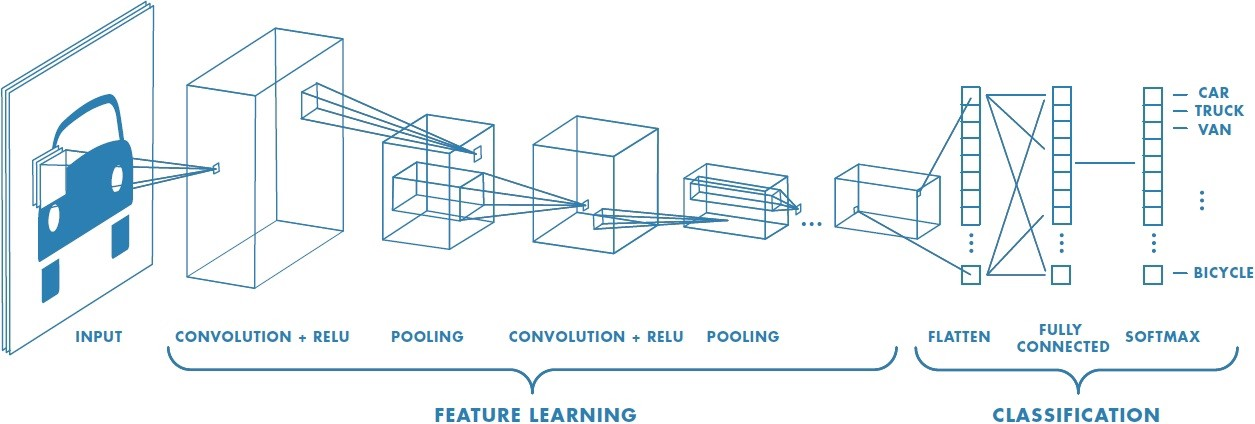
\includegraphics[width=0.5\columnwidth]{Image/CNN.jpeg}
\caption[CNNpic1]{ Basic convolutional neural network architecture \cite{CNNpic}}
\label{fig:BoxesAndArrowsAreNice}
\end{center}
\end{figure}

In short, convolutional networks are a subset of neural networks, they are also made up of neurons that have learnable weights and biases. In CNN, the network will process the input train data through a series of convolution layers with filters (Kernals), Pooling, fully connected layers (FC), etc... and then perform the classification with help of function like softmax at the end.\cite{CNN} Convolution in this case is the first layers of the network, which apply filters to the input tensor. It can extract the features from the image by preserving the relation between pixels. The pooling layer then use to reduce the numbers of parameters, which is very useful for example when the input image is large. 
\subsubsection{VGG-net}
The VGG-net is a deep convolutional neural network for object recognition developed and trained by  Visual Geometry Group from Oxford.\cite{2014arXiv1409.1556S} "It was demonstrated that the representation depth is beneficial for the classification accuracy, and that state-of-the-ar performance on the ImageNet challenge dataset can be achieved using a conventional CNN architecture with substantially increased depth. " (VGG-net authors)
Until today, VGG-net still remain one of the most cost-effective CNN- architecture because of the short required training and it relative powerful performance.

\begin{figure}[ht]
\begin{center}
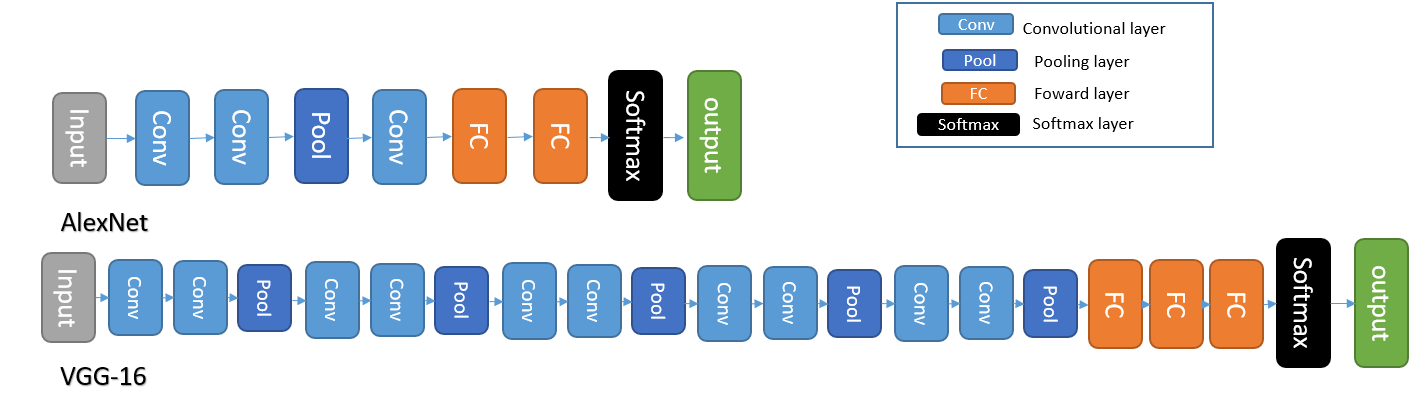
\includegraphics[width=1\columnwidth]{Image/alexvgg.PNG}
\caption[CNNpic1]{ Architecture Comparition between Alexnet and VGG-16  \cite{CNNpic}}
\label{fig:BoxesAndArrowsAreNice}
\end{center}
\end{figure}

\subsection{Active learning}
Even with the most advance neural network architecture, it is still impossible to achieve a acceptable result without a sufficient amount of labeled data. However, the acquisition of labeled data for new tasks is both challenging and costly. In such case, active learning can be used to lower the cost of annotation without sacrificing. The motivation behind active learning focus on, given a pool of unlabeled data and a limited annotation-budget, there must exist an optimal way to query the best sub-set of it for label, such that sub-set queried by active learning would significantly outperform a random selected sub-set. The problem of active learning in image classification can be formulated as follow. Given  an unlabeled data-set of $X^U$ and a labeled data-set of $X^L$ , the algorithm need to take $k$ samples from $X^U$, query the correspond label from an oracle and add them to $X^L$ in order to minimize the classification error of a model trained on $X^L$.
\subsection{Batch-mode Active learning}
In most active learning research, the queries are selected one at a time, i.e serial. However, such method is sometimes very very inefficient and time-consuming \cite{activelearningbook}. In many cases, there would be multiple annotators working on different labeling workstations at the same time span on a network and the query speed is not fast enough to catch up with the labeling speed. In such cases, active learning method that selecting queries in serial may be inefficient and this has given rise to batch-mode active learning. Batch-mode active learning allow the learner to query instances in groups, which proof to be more effective for parallel labeling or network with long training time. The goal of batch-mode active learning is to select an optimal query set $\mathbf{Q}$ which performance is comparable with serial selecting. Although, it is very challenging since the active learner fails to consider the overlap in information content among the selected instances and for batch. There has been several research studies that address this problem \cite{Discriminativebatchmode} and various of proposed method to combat this \cite{6912976}. For the most part, these approaches has show a better result then random batch sampling, but still not comparable to serial query. \cite{activelearningbook}
\subsection{Active learning in image classification}
Active learning has been applied and achieved a considerable amounts of success in different area of machine learning, from speech recognition to object detection \cite{workshop}. As for image classification, the key idea of active learning revolve around achieve greater accuracy with fewest number of labeled training samples. One of the most common approach is uncertainty base active learning, where the learner select instances based on the classifier uncertainty. However, we can also perform selection base on dissimilarity between instances, i.e distances between data points or by reducing the expected error reduction by simulate the label outcome of each instances. 


\subsection{Uncertainty base active learning}
One of the most basis and simplest method in active learning is to query base on the uncertainty of the classifier. For this method there are 3 main way to determine the selection criteria: Least confidence (LC), margin sampling (MS) \cite{roy2001toward}, and entropy \cite{shannon1948mathematical}. 
\subsubsection{Least confidence selection}
This method query instances one by one by select the unlabeled instances $x_i$ that have lowest score given by the function $max(p(y_j|x_i))$, which is the probability of instance $x_i$ belongs to class $y_j$.
\begin{equation}
    x^{LC}_i =\underset{x \in X^U}{argmin} ( max(p(y_j|x_i)))
\end{equation}
\subsubsection{Margin sampling selection}
This strategy pick the sample with the smallest probability different of the top two class predictions $y_1$ and $y_2$.
\begin{equation}
    x^{MS}_i =\underset{x \in X^U}{argmin} ( (p(y_1|x_i)- p(y_2|x_i)))
\end{equation} 
\subsubsection{Entropy selection}
The selection takes all class label probabilities into consideration to measure uncertainty and select the one with largest class prediction information entropy.
\begin{equation}
    x^{entropy}_i =\underset{x \in X^U}{argmax} (\sum_{j}p(y_j|x_i)log(p(y_j|x_i))
\end{equation} 
\subsection{Deep Bayesian Active Learning}
Deep Bayesian Active Learning(BALD) \citet{GalIG17}, is one of the more sophisticated uncertainty base method of active learning designed for deep CNN. The method make use of the Bayesian equivalent of CNN\citet{gal2015bayesian}, which are CNNs with prior probability distribution placed over a set of model parameters $\omega = {W_1, ... , W_L}$. To achieve this, we applied stochastic regularization techniques such as dropout where dropout can be interpreted as a variational Bayesian approximation. The prediction probabilities of an instance in this case will be:
\begin{equation}
    p(y_j|x_i) = \frac{1}{T} \sum_{t=1}^Tp(y_j|x_i, \hat{\omega}_t)
\end{equation} 
with T is the number of different outcome of the neural network affected by $\hat{\omega{_t}}$ with $\hat{\omega{_t}} \sim q^{*}_\theta(\omega)$ where  $q^{*}_\theta(\omega)$ is the dropout distribution. The selection function of this method can be written as follows:
\begin{equation}
    x^{BALD}_i =\underset{x \in X^U}{argmin} (- log(p(y_j|x_i)) + \frac{1}{T}\sum_{t=1}^Tp(y_j|x_i,\hat{\omega}_t)log(p(y_j|x_i,\hat{\omega}_t)))
\end{equation}
where $p(y_j|x_i, \hat{\omega}_t)$ is the prediction probability of each CNN with different weight parameters affected by dropout.  
\subsection{Deep Bayesian Active Learning}    
\subsection{Cost-effective active learning}
\begin{equation}
    S^{A}_{x} = \begin{bmatrix}
       |5| \\[0.3em]
       \frac{5}{6} \\[0.3em]
       0           
     \end{bmatrix}
\end{equation}
\subsection{Criteria switching active learning}
As previous mentioned, active learning is st 
\begin{figure}[ht]
\begin{center}
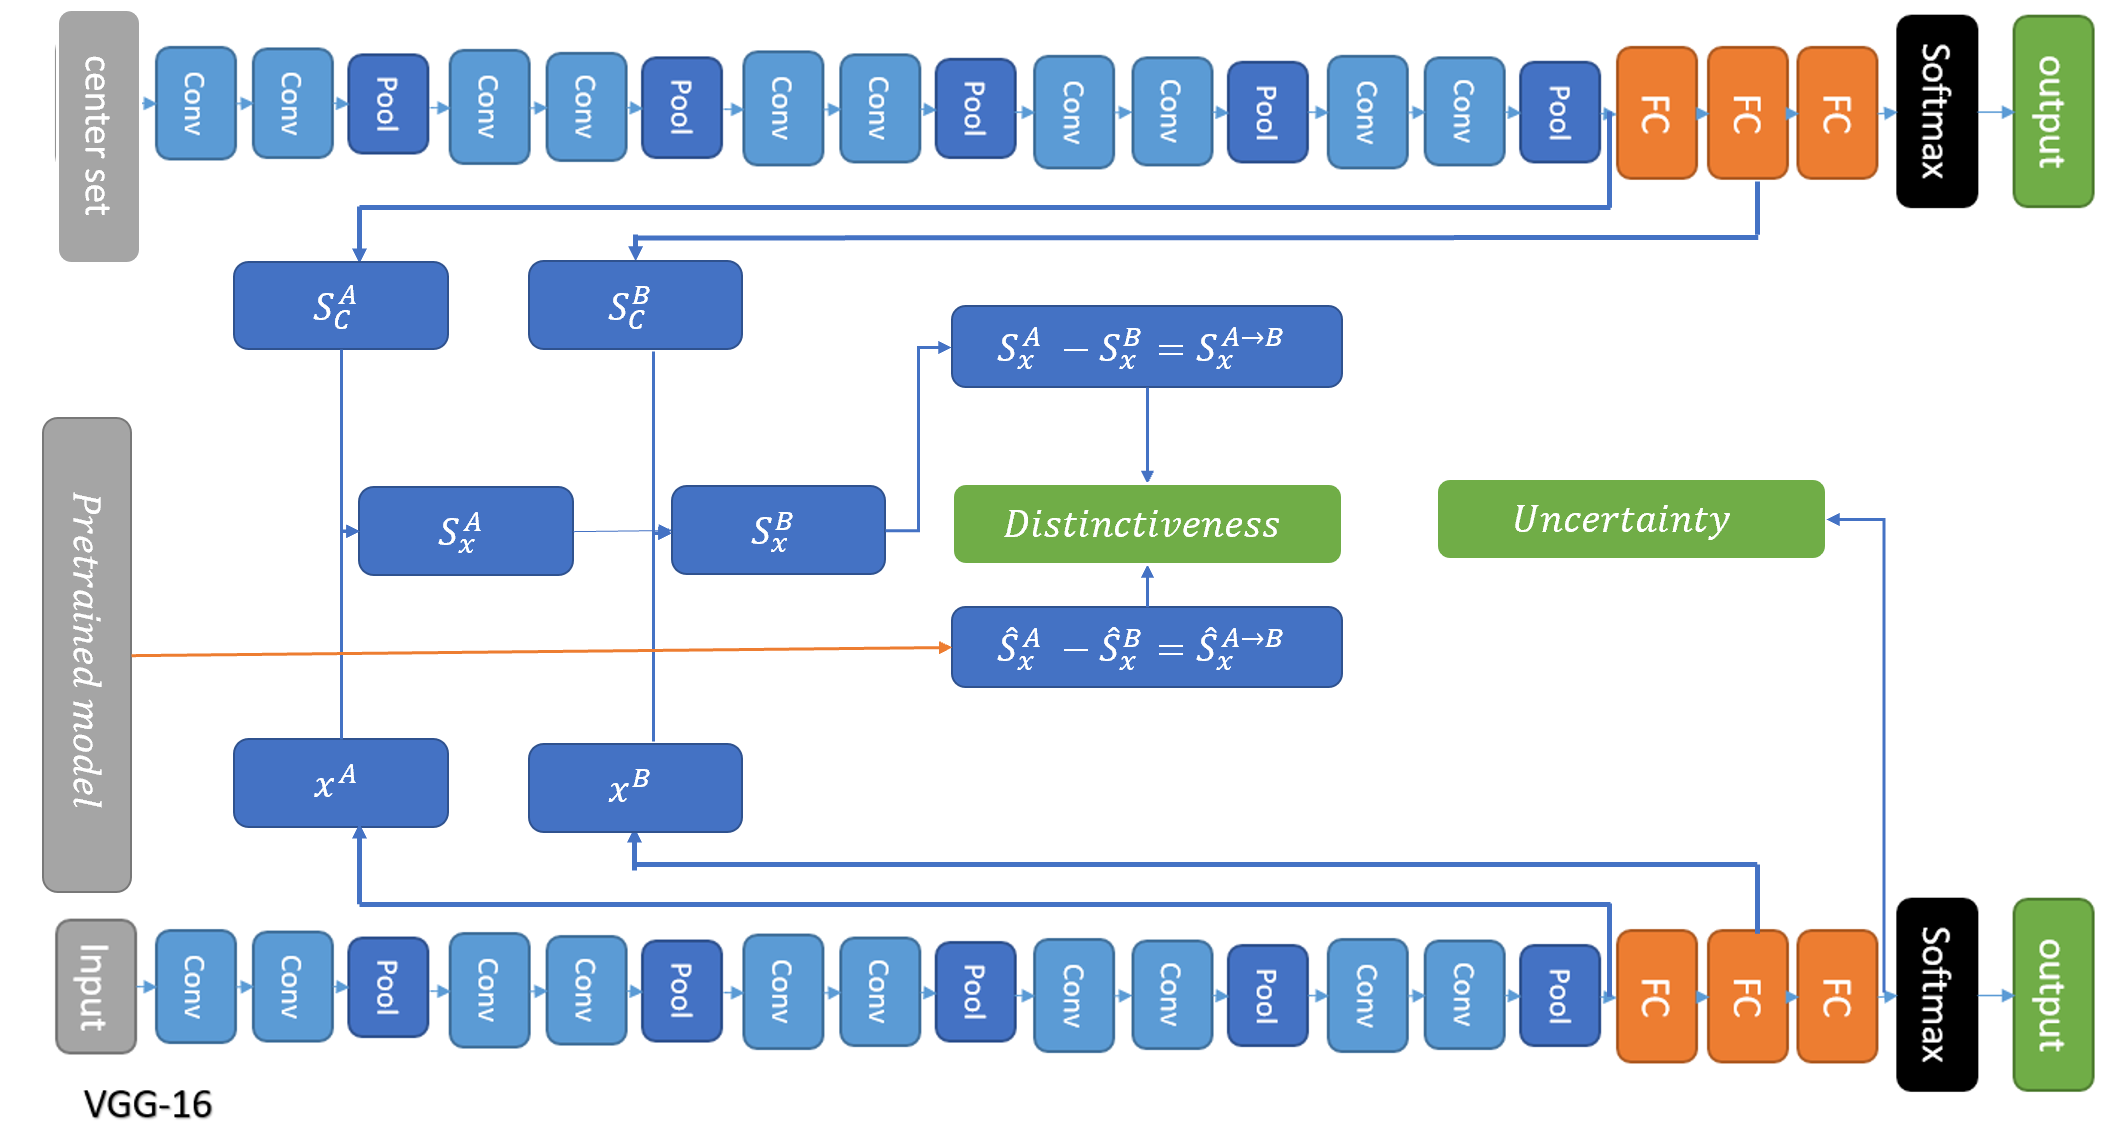
\includegraphics[width=1\columnwidth]{Image/vgg.PNG}
\caption[vgg]{ cost effective }
\label{fig:BoxesAndArrowsAreNice}
\end{center}
\end{figure}
\cite{costeffective}
\cite{costeffective2}
\subsection{Core-set approach Active learning}
\label{sec:no1}

%The background theory depth and breadth depends on the depth needed to understand your project in the different disciplines that your project crosses.  It is not a place to just write about everything you know that is vaguely connected to your project. The theory is here to help the reader that does not know the theoretical basis of your work so that he/she can gain sufficient understanding to understand your contributions. In particular, the theory section provides an opportunity to introduce terminology that can later be used without disturbing the text with a definition.  In some cases it will be more appropriate to have a separate section for different theory. However, watch that you don't end up with too short sections. Subsections may also be used to separate different background theory. 

%When introducing techniques or results, always reference the source. Be careful to reference the original contributor of a technique and not just someone who happens to use the technique. For relevant results to your work, you would want to look particularly at newer results so that you have referenced the most up-to-date work in your area. If you don't have the source handy when writing, mark the test that a reference is needed and add it later. 

%Web pages are not reliable sources --- they might be there one day and removed the next; and thus should be avoided, if possible. A verbal discussion is not a source and should not be referenced or described in the text.  

%The bulk of citations in the report will appear in section~\ref{cit}. However, you will often need to introduce some terminology and key citations already in this chapter. 

%You can cite a paper in the following manners: 



\noindent
{\bf Introducing tables in the report: }\\

\begin{table}[htbp]
\begin{center}
\begin{tabular}{|c|c|c|c|c|}\hline\hline
This & is & a & nice & table\\\hline
This & is & a & nice & table\\\hline\hline
\end{tabular}
\caption{Example Table}
\end{center}
\label{tab:ExampleTable}
\end{table}%

As you can see from Table \ref{tab:ExampleTable}, tables are nice. However, again, you need to discuss the contents of the table in the text. You don't need to describe every entry but draw the authors attention to what is important for he/she to glean from the table. 

\section{Structured Literature Review Protocol}

What is this ???

\section{Related work}
\label{sec:no2}

\subsection{Uncertainty base active learning}
\subsection{Distance base active learning}
\subsection{Cost-effective active learning}
